\chapter{Turn-taking decision module: the Scheduler}

\label{ch:architecture}

\section{Description}
	\subsection{Overview}
    
    	A new incremental dialogue system architecture is introduced in this Chapter. The five modules forming the dialogue chain (see Chapter \ref{ch:soadialogue}) are split in two groups: those forming the \textit{client} and those constituting the \textit{service}. The ASR and the TTS are necessarily included in the client and the  DM in the service. The NLU and the NLG can fit in both categories. This terminology has been borrowed to the computer network field \cite{Israel1978} where the client can refer to the user and to the application that interacts directly with the user in order to gather useful data for the interaction at the same time. Similarly, the server refers to the application that is in charge of handling user's requests, as well as the remote machine it is deployed on. In the case of dialogue systems, both parts can be embedded in the same device and they can also be distributed in two different machines.
        
        Viewing traditional dialogue systems from this point of view translates into a ping-pong game, where the client sends a request which is processed by the service, and the latter sends a response back. The question tackled here is how to break this rigid mechanism in order to make the system able to process the user's speech incrementally. This chapter shows how, by starting from this new view of dialogue systems instead of the sequential one (dialogue chain), an incremental dialogue system can be derived from a traditional one at minimal cost. In the resulting architecture, the turn-taking decision maker is separated from the DM allowing an autonomous control of the nature and timing of the incremental behaviour.
        
        As illustrated in Fig. \ref{fig:archioverview}, a new interface is inserted between the client and the service \cite{Khouzaimi2014a}. This new module is called the \textit{Scheduler} (this denomination is borrowed from \cite{Laroche2010a}). It can be deployed on the same machine as the client, as the service or in a dedicated server. The objective is to make the set \{Scheduler+service\} behave like an incremental dialogue system from the client's point of view, without modifying the initial functioning of the service. Therefore, this provides a framework that can transform any dialogue system in its incremental version just by adding a new layer.
				
        This alternative way of designing incremental dialogue systems also has the theoretical advantage of clearly separating turn-taking management from the rest. Turn-taking strategies are conceived and formalised independently from the task at hand: they can be reused as they are for different tasks. They can also be manipulated separately and combined in order to form new complex strategies given specific rules. As a consequence, this kind of architecture has the advantage of being more modular. As it will be seen along this thesis, turn-taking strategies will be implemented exclusively in the Scheduler (the rest of the system remaining the same). Our ultimate goal is to make this module learn optimal turn-taking behaviours by itself.
        
     	\begin{figure*}[t]
          \centering
          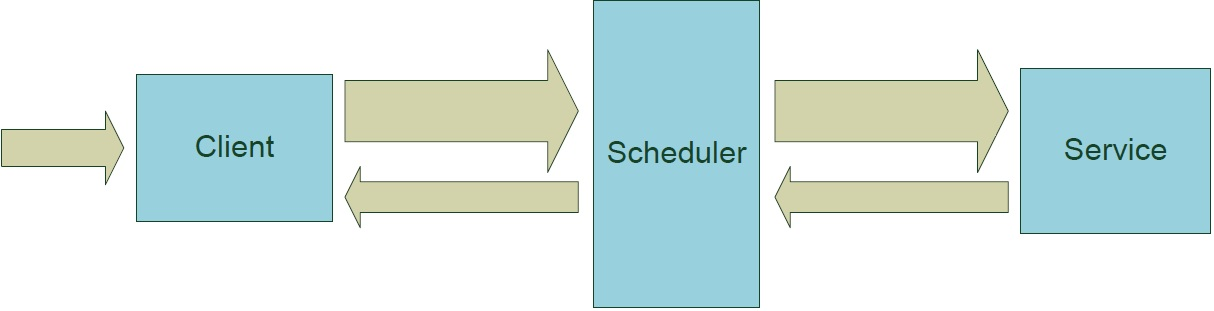
\includegraphics[scale=0.4]{figures/ClientSchedService.jpg}
          \caption{The Scheduler: an interface between the client and the service}
          \label{fig:archioverview}
        \end{figure*}
        
    \subsection{Time sharing}
    
    	In traditional dialogue systems, time is shared in an ordered and clear manner. The dialogue is a simple sequence of turns $T^1,T^2...$, a turn being the time interval in which a user's utterance followed by the system's corresponding response takes place, or the opposite (depending whether the system adopts a user initiative or a system initiative strategy at each turn). For illustration and to simplify the notation, the system used here is supposed to belong to the first category, therefore, each turn is divided into two smaller time intervals, the user turn $T^{k,U}$ and the system turn $T^{k,S}$: $T^k = T^{k,U} \cup T^{k,S}$ (Fig. \ref{fig:timeshare}).
        
        In this chapter, a few conditions are defined to precisely describe time allocation between the system and the user. The \textit{activation time} of a condition refers to the exact moment when it goes from false to true. \textit{EndTurnCond} is the condition that ends a user turn, it is generally assimilated to a long silence \cite{Raux2008,Wlodarczak2013}.
        
        \begin{figure*}[t]
          \centering
          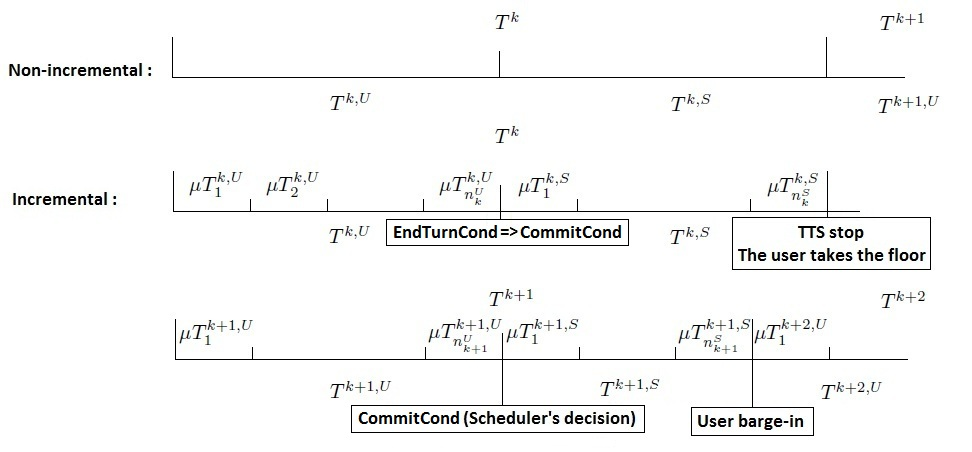
\includegraphics[scale=0.6]{figures/Timeline.jpg}
          \caption{Time sharing in traditional and incremental settings}
          \label{fig:timeshare}
        \end{figure*}
        
        In incremental settings, this time sharing formalism does not hold anymore and a new condition should be defined: \textit{EndMicroTurnCond} (with \textit{EndTurnCond} $\Rightarrow$ \textit{EndMicroTurnCond}). The time interval separating two activation times of \textit{EndMicroTurnCond} is called a \textit{micro-turn}. As a consequence, the turn $T^{k,U}$ can be divided into $n^{k,U}$ micro-turns $\mu T^{k,U}_i$: $T^{k,U} = \bigcup_{i=1}^{n^{k,U}} \mu T^{k,U}_i$. The $p^{th}$ \textit{sub-turn} of turn $T^{k,U}$ is defined as $T^{k,U}_p = \bigcup_{i=1}^p \mu T^{k,U}_i$.
        
        The request that the user makes during $T^{k,U}$ is referred to as $Req^k$ and the corresponding response is $Resp^k$. This architecture does not process incremental units like in \cite{Schlangen2011}, instead, at each new micro-turn, it will take the whole information available since the beginning of the turn\footnote{This way of managing incremental dialogue is called \textit{restart incremental} in \cite{Schlangen2011}.} (at the $p^{th}$ micro-turn, all what the user uttered during $T^{k,U}_p$). This \textit{partial request} is called $Req^k_p$.
        
    \subsection{The Scheduler}
    
    	\begin{figure*}[htp]
          \centering
          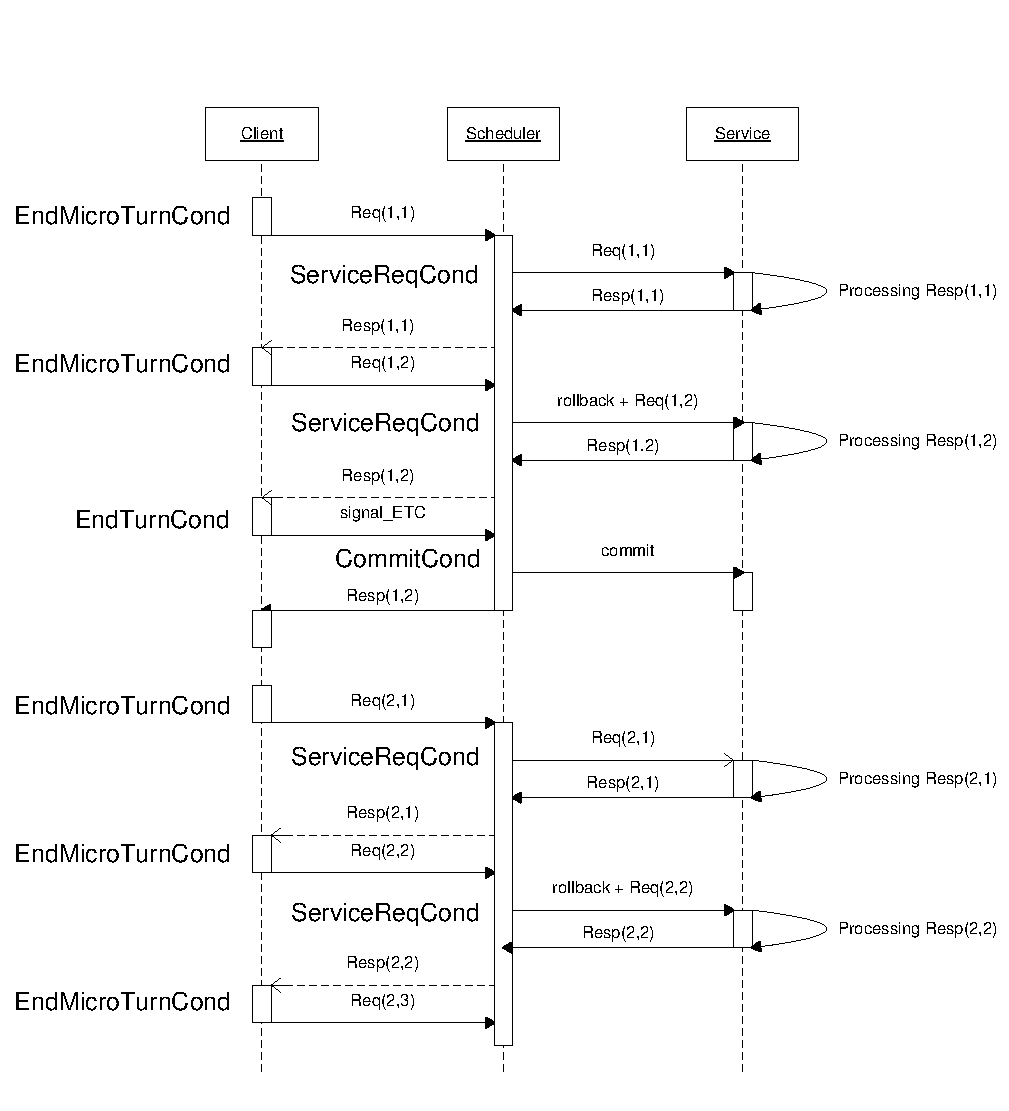
\includegraphics[scale=0.8]{figures/SchedulerDiagEng.pdf}
          \caption{Incremental behaviour with the Scheduler}
          \label{fig:schedchrono}
        \end{figure*}
    
    	During the $p^{th}$ micro-turn of the $k^{th}$ user turn, the client sends $Req^k_p$ to the Scheduler. The latter has to decide whether to send it to the service or not and the corresponding condition is called \textit{ServiceReqCond}. A good example is \textit{ServiceReqCond} = ($Req^k_p \neq Req^k_{p-1}$) as sending the same request twice is useless. Then, the service provides the corresponding response $Resp^k_p$ and the Scheduler stores it. The key idea of this architecture is that the Scheduler decides whether to retrieve this response to the client (making it take the floor through the TTS) or not (waiting for more information to come from the client). This decision can also be forced by the client when sending an end of turn signal signal\_ETC, like a long enough silence for instance. The most interesting fact about the Scheduler is that it is able to decide when to take the floor without waiting for signal\_ETC, the corresponding condition is called \textit{CommitCond}. The Scheduler functioning over time is illustrated in Fig. \ref{fig:schedchrono} (dashed arrows represent the Scheduler's response to the client since they may or may not take place, given the Scheduler's decision to commit or not).
        
	\begin{table*}[htp]
		\begin{center}
		\begin{tabular}{|c|c|c|c|c|}
			 \hline
			 \textbf{Turn} & \textbf{User sub-turn} & \textbf{Input} & \textbf{Real context} & \textbf{Simulation context} \\
			 \hline
			 $T^1$ & $T^{1,U}_1$ & $Req^1_1$ & ctxt($T^0$) & ctxt($T^0 + T^{1,U}_1$) \\
						 & $T^{1,U}_2$ & $Req^1_2$ & ctxt($T^0$) & ctxt($T^0 + T^{1,U}_2$) \\
						 &    ...     &     ...     & ctxt($T^0$) & ... \\
						 & $T^{1,U}_{n^{1,U}}$ & $Req^1_{n^{1,U}}$ & ctxt($T^0$) & ctxt($T^0 + T^{1,U}_{n^{1,U}}$) \\
			 \hline
						 & \multicolumn{3}{c}{\multirow{2}{*}{\textbf{COMMIT:} $ ctxt(T^1) = ctxt(T^0 + T^{1,U}_{n^{1,U}}) $}} & \\
						 & \multicolumn{3}{c}{} & \\
			 \hline
			 $T^2$ & $T^{2,U}_1$ & $Req^2_1$ & ctxt($T^1$) & ctxt($T^1 + T^{2,U}_1$) \\
						 &    ...     &     ...     & ctxt($T^1$) & ... \\
			 \hline
		\end{tabular}
	        \end{center}
	        \caption{A double context: the real context and the simulation context.}
	        \label{tab:contextchrono}
        \end{table*}
        
        Nevertheless, this approach raises on technical problem. Most of the requests that are made to the service are only aimed to see what would be its response for certain partial utterances and they are discarded right after. However, they might modify the dialogue state in the service which is a side effect to be avoided. As a consequence, two dialogue contexts are maintained:
        
        \begin{itemize}
           	\item \textbf{The real context:} The dialogue context as traditionally used in dialogue systems. Contains the data and the variables that are aimed to last and be used in the rest of the dialogue.
        	\item \textbf{The simulated context:} A copy of the real context, at the $p^{th}$ micro-turn, $Resp^k_p$ could be useful for the dialogue or not. Therefore, only this context is modified at the first place, the Scheduler decides later whether to keep the changes in the real context or not.
        \end{itemize}
        
        These dialogue contexts are managed by two actions performed by the Scheduler:
        
        \begin{itemize}
        	\item \textbf{Commit:} The Scheduler commits to a partial request and the corresponding response when it decides to deliver the latter to the client, hence taking the floor immediately and not waiting for any further information. In that case, the simulated context is saved into the real context (thus becoming the new reference).
            \item \textbf{Cancel or rollback:} The scheduler cancels the context changes when it decides to discard the last response obtained from the service and that a new - potentially more complete - partial request is received from the client (as shown in Figure \ref{fig:schedchrono}). In that case, the real context is copied into the simulated one, rollbacking it to its original state.
        \end{itemize}
 
 		The way the real and the simulated context are managed through the commit and the cancel actions is illustrated in Table \ref{tab:contextchrono}.

        
\section{Illustration}

        As a proof of concept, this section describes two instanciations of the previous abstract architecture, both in the case of a textual and a spoken dialogue system.

	\subsection{A textual dialogue system: CFAsT}
    
    	\begin{figure*}[ht]
          \centering
          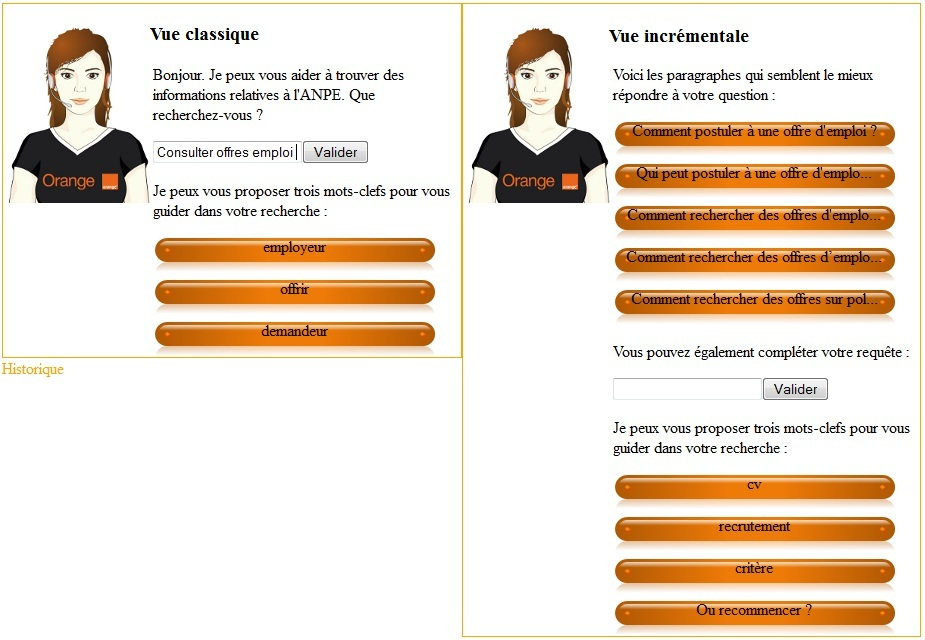
\includegraphics[scale=0.6]{figures/CFAsTIncr.jpg}
          \caption{The incremental version of the CFAsT project. The traditional view is represented on the left and the new incremental one is depicted on the left.}
          \label{fig:CFAsTIncr}
        \end{figure*}
        
        CFAsT stands for Content Finder AssistanT. This application, developed at Orange Labs \cite{Laroche2014,Laroche2015}, is aimed at automatically generating virutal assistants that help the user efficiently find specific content in databases (given as input). At each dialogue turn, the user provides some new information about his target and by using a keyword spotting algorithm, the system keeps narrowing the set of possibilites. The interface is made of a text box with a \textit{validate} button. The dialogue service is deployed as a web service on a servlet container and the client is a javascript web page loaded on the user's browser.
        
        In order to make it incremental, a Scheduler has been deployed as a servlet on the same container as the service and the javascript requests have been re-targeted towards it (the service is no longer directly visible by the client). Moreover, as discussed earlier, the dialogue context in the service have been duplicated. In this setup, \textit{EndTurnCond} corresponds to the event of clicking on \textit{validate} (or hitting the carriage return). A word-based micro-turn configuration has been implemented, therefore, \textit{EndMicroTurnCond} is the action of hitting the space bar. Each request being different from the previous one, they should all be sent to the service, thus, \textit{ServiceReqCond} is true all the time.
        
        This implementation is aimed to provide a first proof of concept of the methodology introduced here. However, signal\_ETC = \textit{CommitCond} = \textit{EndTurnCond} (the Scheduler never takes commit decisions by itself). The resulting behaviour presents a noteworthy similarity with autocompletion in search engines. The most staightforward way this mechanism is implemented is by continuously proposing several hypotheses regarding what would the complete request be, regarding the partial request typed so far. This does not require any request to the search engine itself (which can be viewed as the Service in the architecture introduced here). Another implementation (which lately started to be deployed) is by continuously updating the search result which is quite similar to what the transformed CFAsT achieves.
    
    \subsection{A spoken dialogue system: Dictanum}
    
    	Number dictation is an activity that can be encountered in several kinds of applicative domains: phone numbers, credit cards...Analysing human conversations in such situations shows that the number at hand is often broken into small pieces (a few digits each) and a confirmation follows each one of them. Therefore, the number is incrementally grounded so that in the case of a misunderstanding, only the last dictated part has to be repeated. Traditional dialogue systems behave differently as they ask the user to enter the whole number at once. This translates into long and tedious dialogues as only one minor mistake is enough to make the user repeat the number from the beginning, often for several times. For example:
        
        \begin{dialogue}
        	\speak{SYSTEM} Welcome to the Dictanum service. Please dictate your number.
            \speak{USER} 01 45 65 79 98.
            \speak{SYSTEM} The dictated number is 01 45 67 79 98. Is that correct?
            \speak{USER} No.
            \speak{SYSTEM} Sorry. Let us try again. Please dictate your number.
            \speak{USER} 01 45 65 79 98.
            \speak{SYSTEM} The dictated number is 01 47 65 79 98. Is that correct?
            \speak{USER} No.
            \speak{SYSTEM} Sorry. Let us try again. Please dictate your number. \\
            $\left[...\right]$ \textit{(given that the user is patient enough not to hang up)}
            \speak{SYSTEM} The dictated number is 01 45 65 79 98. Is that correct?
            \speak{USER} Yes.
            \speak{SYSTEM} Thank you for using Dictanum. Bye.
        \end{dialogue}
        
        With incremental dialogue processing, it is possible to design a strategy that is closer to the human behaviour. To show that, a number dictation dialogue system called Dictanum (described in \cite{Khouzaimi2014c})  has been implemented using Disserto. It performs turn-based dialogue hence asking the user for the whole number at once. Here, the client is a web page displayed on the browser that uses Google API for both the ASR and the TTS tasks and the service is a servlet deployed on a servlet container.
        
        Afterwards, the approach introduced here has been used to build the incremental version of the system (like in the case of the CFAsT application, the Scheduler has been deployed as a servlet on the same container as the service). To do so, two silence duration thresholds have been defined: the short silence threshold $\delta_s$ and the long one $\Delta_s$ ($\delta_s \leq \Delta_s$). \textit{EndMicroTurnCond} is triggered when a short silence is detected and similarly, \textit{EndTurnCond} corresponds to long silences. A feedback is delivered to the user in the case of a short silence (repeating the last 4 digits). If the user ignores the feedback and keeps dictating his number, the system keeps on adding digits to its list, however, if the user starts his next utterance with \textit{No}, the feedback content is deleted from the number. Here is a dialogue example:
        
        \begin{dialogue}
       	    \speak{SYSTEM} Welcome to the Dictanum service. Please dictate your number.
            \speak{USER} 01 45 \textit{(short silence)}
            \speak{SYSTEM} 01 45
            \speak{USER} 65 79 \textit{(short silence)}
            \speak{SYSTEM} 67 79
            \speak{USER} No, 65 79 \textit{(long silence)}
            \speak{SYSTEM} Sorry, 65 79
            \speak{USER} 98 \textit{(short silence)}
            \speak{SYSTEM} 98
            \speak{USER} ... \textit{(long silence)}
            \speak{SYSTEM} The dictated number is 01 45 65 79 98. Is that correct?
            \speak{USER} Yes.
            \speak{SYSTEM} Thank you for using Dictanum. Bye.
        \end{dialogue}

        It is interesing to notice that if $\delta_s = \Delta_s$, the user is likely to dictate his number in one shot, never waiting for a feedback. Therefore, moving $\delta_s$ between 0 and $\Delta_s$ creates a continuum between the traditional and the incremental version.
        
        Dictanum also offers the possibility for the user to interrupt the system during the final feedback, in order to make local corrections. To do that, this feedback is sent to the TTS in the following format: \textit{The dictated number is 01 <sep> 45 <sep> 65 <sep> 79 <sep> 98. Is that correct?}. The latter pronounces the sentence chunk after chunk (chunks are delimited using the separator \textit{<sep>}), each chunk lasting for the same number of micro-turns. This leads to the following kind of strategy:
        
        \begin{dialogue}
            \speak{SYSTEM} The dictated number is: 01 45 67...
            \speak{USER} No, 65.
            \speak{SYSTEM} Sorry. The dictated number is 01 45 65 79 98. Is that right?
            \speak{USER} Yes.
            \speak{SYSTEM} Thank you for using Dictanum. Bye.
        \end{dialogue}
    
\section{Discussion}

	\subsection{Levels of incrementality}
    
    	Dialogue systems can be classified in four categories given the way they integrate incremental behaviour. The first category is made of traditional systems \cite{CLASSiCd64}. Then comes the second category where traditional systems locally implements a few incremental behaviours. For instance, in \cite{El-Asri2014a}, the system enumerates a list of options and the user selects the one that fits him best by uttering \textit{Yes} or \textit{Ok} for example (REF\_RAW in the taxonomy introduced in Chap. \ref{ch:taxonomy}). The architecture introduced in this thesis belongs to the third category where incremental behaviour is obtained based on modules that are innately non-incremental (the service in our case). Other examples are described in \cite{Selfridge2012a} and \cite{Hastie2013}. Finally, the fourth category is made of incremental dialogue systems that are constituted of fully-incremental modules. In \cite{Schlangen2011}, an abstract model for incremental architectures is presented where all the categories can fit, but the work that has been pursued by the authors and their research groups later on goes along with the spirit of this last category.
		
		Categories 2, 3 and 4 embed different features related to incremental behaviour (summarised in Fig. \ref{tab:incrclassif}):

                \begin{itemize}
                  \item \textbf{TTS interruption after input analysis:} The user has the ability to interrupt the system (BARGE\_IN\_RESP from the user's side) but also to perform brief feedback (BACKCHANNEL or FEEDBACK TTP from the user's side) without interrupting the system's sentence. All categories except the first one can easily embed this feature.
                  \item \textbf{Link interruption time with TTS:} Useful for simulating REF TTP (REF\_IMPL, REF\_RAW and REF\_INTERP from the user's side). This has been successfully implemented in a system that belongs to the second category in \cite{El-Asri2014a}. Therefore, it can also be implemented in systems with a higher degree of incrementality (categories 3 and 4).
                  \item \textbf{User interruption by the system:} As it will be shown in the rest of this thesis, interrupting the user can improve the dialogue efficiency in some cases (BARGE\_- IN\_RESP from the system's side). To do so, the sytem at hand must offer real incremental capacities which is the case for categories 3 and 4 only.
                  \item \textbf{Better reactivity:} One of the main advantages of incremental processing is delivering responses in a quicker fashion since the processing of the user's request starts earlier. Again, real incremental abilities are required which makes it a property that is specific to categories 3 and 4 exclusively. This feature is particularly useful to achieve accurate end point detection (END\_POINT from the system's side).
                  \item \textbf{Optimal processing cost:} The third category processes the user's request in a restart incremental way (sending the whole partial utterance at each new micro-turn). This is not optimal as it is possible to process it chunk by chunk. Therefore, this is an advantage that category 4 offers over all the others.
                \end{itemize}

	\subsection{Enhancing a traditional dialogue system's turn-taking abilities at a low cost}
    
             Adopting the sequential paradigm described in Chapter \ref{ch:soadialogue} is a natural way of designing incremental dialogue systems \cite{Schlangen2011}. The dialogue chain is kept unchanged, however, a substantial amount of work has to be done in order to design an incremental version of each one of the modules. The approach introduced in this chapter makes it possible to build an incremental dialogue system starting from a traditional one instead of starting from scratch. Therefore, the development cost is significantly reduced and moreover, the resulting incremental dialogue system benefits from all the experience and the adjustments embedded in the original dialogue system. In the following, the differences between the two approaches are reviewed as well as the elements that are simplified with the new approach and the price one has to pay to adopt it.

             Incremental ASR is a prerequisit for the implementation of a Scheduler-based architecture. Therefore, it is not simplified by this approach and an inaccurate, slow or unstable ASR module still hurts the dialogue quality in the same way. In terms of NLU, two cases have to be distinguished: putting the Scheduler before the NLU or after it. In the first case, it does not make sense to use an incremental NLU as the Scheduler proceeds on a restart incremental fashion (sending the whole user's partial utterance at each micro-turn). However, in the second case, it is possible to benefit from the advantages of incremental NLU (forming concepts in a real incremental way resulting in more efficient processing). In that case, the Scheduler receives a sequence of potentially unstable sets of concepts.

             The core difference between both approaches resides in the DM task. In a full-incremental architecture, dialogue act and turn-taking decisions are intertwined. The DM receives the input concepts chunk by chunk, and at each micro-turn, the new information can be viewed as the continuity of what has been understood so far, or as a signal pushing the DM to revoke the current hypothesis before taking a new action. In the Scheduler-based approach, as the restart incremental paradigm is adopted, the revoke mecanism is intrinsicly implemented as it is performed beforehand (the ASR changing its best hypothesis is a case of revoke).

             Incremental NLG does not make sense in the frame proposed here as the Scheduler can only retrieve full dialogue acts that have been precomputed by the service. As a consequence, the system can change its mind about the utterance currently uttered but it can only generate a new dialogue act from scratch with is potentially not related to the previous one. Nevertheless, as discussed in Chapter \ref{ch:soadialogue}, this is not a major problem when it comes to spoken dialogue systems relying on voice as the only interaction modality. It is mostly used when the system produces comments about a moving object or situation it is observing \cite{Baumann2013}.

             Finally, as far as the TTS task is concerned, the same remark as for the NLG can be made. However, it can be interesting to give the Scheduler the power to stop the TTS. This is particularly interesting when the DM decides to revoke its current belief.

             \begin{table*}[!ht]
      	     \footnotesize
             \centering
             \begin{tabular}{|c|c|c|c|c|}
               \hline
               \textbf{Features}	& \textbf{Category 1} & \textbf{Category 2} & \textbf{Category 3} & \textbf{Category 4} \\
               \hline
               TTS interruption after input analysis & - & + & + & + \\
               \hline
               Link interruption time with TTS & - & + & + & + \\
               \hline
               User interruption by the system & - & - & + & + \\
               \hline
               Better reactivity & - & - & + & + \\
               \hline
               Optimal processing cost & - & - & - & + \\
               \hline
             \end{tabular}
             \caption{Available features for dialogue systems given the way they integrate incrementality}
             \label{tab:incrclassif}
             \end{table*}
